%!TEX TS-program = xelatex
\documentclass[12pt, a4paper]{article} 

%%%%%%%%%% Математика %%%%%%%%%%
\usepackage{amsmath,amsfonts,amssymb,amsthm,mathtools} 
%\mathtoolsset{showonlyrefs=true} % Показывать номера только у тех формул, на которые есть \eqref{} в тексте.
%\usepackage{leqno} % Нумерация формул слева

%%%%%%%%%%%%%%% Шрифты %%%%%%%%%%%
\usepackage{fontspec} % пакет для подгрузки шрифтов
\setmainfont{Arial} % задаёт основной шрифт документа

\defaultfontfeatures{Mapping=tex-text}

% why do we need \newfontfamily:
% http://tex.stackexchange.com/questions/91507/
\newfontfamily{\cyrillicfonttt}{Arial}
\newfontfamily{\cyrillicfont}{Arial}
\newfontfamily{\cyrillicfontsf}{Arial}

\usepackage{unicode-math} % пакет для установки математического шрифта
\setmathfont{Phorssa} % шрифт для математики
% \setmathfont[math-style=ISO]{Asana Math}
% Можно делать смену начертания с помощью разных стилей

% Конкретный символ из конкретного шрифта
% \setmathfont[range=\int]{Neo Euler}

\usepackage{polyglossia} % Пакет, который позволяет подгружать русские буквы
\setdefaultlanguage{russian} % Основной язык документа
\setotherlanguage{english} % Второстепенный язык документа

\author{Кунакбаева Камила} 
\title{Задание 3 домашней 2}
\date{\today}

\begin{document}

\maketitle

\fontspec{Phorssa}{Ты говоришь, что $\sin{\alpha} = \frac{1}{2}$ Может, я и спятил, но я тебе верю. И поэтому я тебя отпущу. И чтобы когда я досчитаю до трех, твоей паршивой, лживой, грязной туши здесь не было... Три!}
\\
\begin{center}
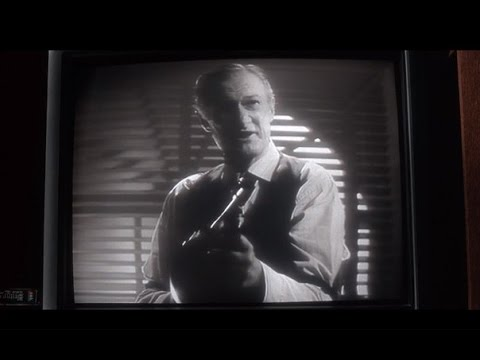
\includegraphics[scale=0.5]{odin_doma.jpg}
\end{center}

\begin{center}
\fontspec{Phorssa}{AHAHAHAHAHAAAA!!!! \\ Merry Christmas and Happy New year.}
\end{center}

\end{document}